\chapter{Backgrounds}

\nocite{DBLP:journals/corr/Lipton15}

As stated in previous chapter, at a high level, our captioning model comprised of a \gls{cnn} which encodes the input image into a fixed-size feature vector and a \gls{lstm} that decodes that feature into sequence of words. This chapter provides backgrounds on machine learning and deep learning, specifically on neural networks for feature extraction and sequence modelling, in order to make the thesis relatively self-contained. Section 1 gives basic introduction on \textit{supervised learning}, the class of machine learing that this thesis deals with. Subsequently, section 2 presents the well-known feed-forward neural networks (or \textit{multilayer perceptrons}). \gls{cnn} is discussed in section 3 together with the algorithm used for training such type of network, \textit{back-propagation}. \gls{rnn} for sequence modelling is presented in section 4. After that, section 5 describes the difficulties and some techniques to overcome challenges when training deep networks. Finally, some standard metrics used in caption evalution research are presented in section 6.

\section{Supervised learning}
\subsection{Overview}
In machine learning, supervised learning is the task of inferring a function from labelled training data \cite{INSR:INSR95_18}. Let $X$ be an input space, $Y$ be the output space. Let's denote $D = \left\{ x_i, y_i\right\}_{i=1}^n$ is the training set of $n$ samples, then $\left(x_i, y_i\right)$ denotes a training sample where $x_i$ is the input and $y_i$ is the desired output (i.e., the groundtruth label). Let's also denote $S = \left\{ x_j, y_j\right\}_{j=1}^m$ as the test set. $D$ and $S$ are disjoint.

The goal of supervised learning is to use training set $D$ to approximate a mapping: $f: X \to Y$ such that the following test error is minimized:
\begin{align}
	\text{Test}_S\left(f\right) \equiv \mathbb{E}_{\left(x, y\right)\sim S}\left[\mathcal{L}\left(f\left(x\right); y\right)\right]
\end{align}

Where $\mathcal{L}$ is a \textit{loss function} that quantifies how well is the induced prediction $\tilde{y}$ given input $x$ to the corresponding groundtruth $y$ in $S$.

\subsection{Probabilistic Classification }


%% ----------------------------------------------------------------
%% SECTION
%%	Feed-forward Neural Network
%% ----------------------------------------------------------------
\section{Feed-forward Neural Networks}
\label{sec:ff}

\subsection{Models of a neuron}

\begin{wrapfigure}{r}{0.35\linewidth}
	\vspace{-20pt} % reduce top space of the figure
	\centering
	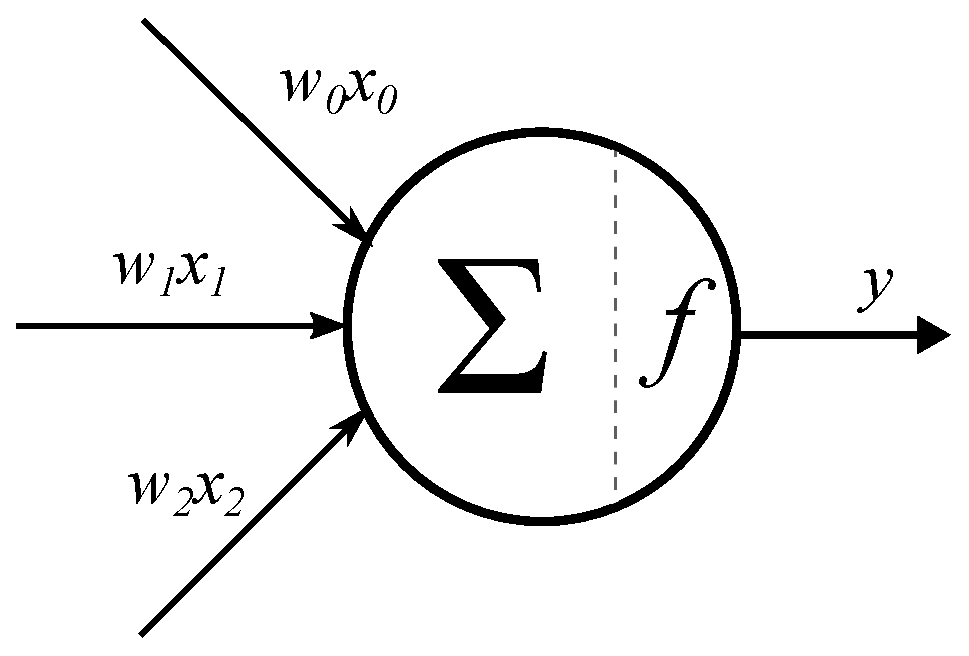
\includegraphics[scale=0.35]{Chapters/Fig/neuron.eps}
	\caption{A single artificial neuron}
	\label{fig:neuron}
	\vspace{-25pt} % decrease bottom space of the figure
\end{wrapfigure}

A neuron is a decisive device which takes several inputs and produces one ouput. Figure \ref{fig:neuron} depicts a neuron which takes three inputs and produces one ouput, where:
\begin{itemize}[noitemsep]
	\item $x_i$: the input to neuron
	\item $w_i$: the weight of input $x_i$
	\item $b$: the bias of neuron
	\item $\sum\left(w_ix_i + b\right)$: the activation of the neuron
	\item $y$: the output of the neuron
\end{itemize}

Here, the learnable parameters are weights $w_i$ and bias $b$. By varying those parameters, we can get different models of decision-making.

There are several types of activation functions often used in deep neural networks. They are listed in Figure \ref{fig:activation-function}
\begin{figure}[h]
	\centering
	\subfigure[Sigmoid function]{%
		$\begin{aligned}
			f\left(z\right) = \frac{1}{1 + e^{-z}}
			\end{aligned}
		$
	}
	\qquad
	\subfigure[Hyperbolic tangent function]{%
		$ \begin{aligned}
			f\left(z\right) = \tanh\left(z\right)
		   \end{aligned}
		$
	}
	\qquad
	\subfigure[Rectified linear function]{%
		$ \begin{aligned}
			f\left(z\right) = max\left(0,z\right)
		   \end{aligned}
		$
		% \includegraphics[width=\linewidth]{Fig/relu.svg}
	}
	\caption{Typical activation functions}
	\label{fig:activation-function}
\end{figure}


\subsection{Feed-forward Neural Network}
Feed-forward neural network (also known as \textit{fully-connected neural network} or \textit{Multilayer perceptrons - MLPs}) is composed of layers of neurons. Figure \ref{fig:ff-net} illustrates typical architecture of such network; the leftmost layer is \textit{input layer}, the rightmost layer is \textit{output layer} and the layers between those two are called \textit{hidden layers}.

\begin{figure}
	\centering
	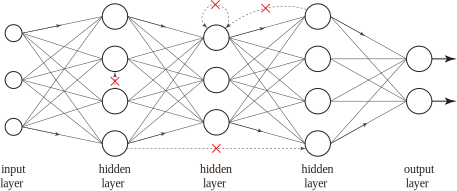
\includegraphics[width=0.85\linewidth]{Chapters/Fig/FFNN.eps}
	\caption[A typical feed-forward network]{A typical feed-forward network consisted of four layers: 1 input layer, 2 hidden layers and one output layer}
	\label{fig:ff-net}
\end{figure}

	\subsubsection{Notation}
	Conventionally, literatures on feed-forward neural network often utilizes the following set of notations
	\begin{itemize}[nosep]
		\item[-] $L$: the number of layers
		\item[-] $l_i$: the $i$-th layer in the network
		\item[-] $W$: the weight matrix
		\item[-] $b$: the bias matrix
	\end{itemize}

	\subsubsection{Connectivity between layers}
	All neurons in layer $\mathit{l_i}$ are connected to every neurons of layer $\mathit{l_{i+1}}$. There is neither backward connection nor connection between neurons of the same layer. The "shortcut" connection between a neuron in layer $\mathit{l_i}$ to any neuron in layer $\mathit{l_j} \left(j > i + 1 \right)$ is also forbidden. 
	
	\subsubsection{Training a feedforward network}
	\nocite{Reed:1998:NSS:552600}
	Formally, a feedforward neural network with $l$ hidden layers is parameterized by $l + 1$ weight matrices $\left( W_0, \dots, W_l\right)$ and $l + 1$ bias vectors $\left( b_1, \dots, b_{l+1}\right)$. Given an input $x$, the feedforward neural network computes an output $z$ as follow:

	\begin{algorithm}
		\begin{algorithmic}
			\State $z_0 \gets x$
			\For {$i$ from $1$ to $l+1$}
				\State $x_i \gets W_{i-1}z_{i-1} + b_i$
				\State $z_i \gets f\left(x_i\right)$
			\EndFor \\
			\Return $z \gets z_l$
		\end{algorithmic}
	\end{algorithm}

	The network is trained by minimizing the training error (assessed by a \textit{loss function}) with respect to the parameters using backpropagation algorithm.
	% The feed-forword neural network has been applied successfully in many classification and regression problems.
	% The goal of a feed-forward network is to approximate a function $f^*$. It defines a mapping $y = f\left(\mathbf{x}; \mathbf{W}; \mathbf{b}\right)$ and learns the values of $\mathbf{W}$ and $\mathbf{b}$ that gives the best approximation.
	
%% ------------------------------------------------------------
%% SECTION
%%     Convolutional Neural Network
%% ------------------------------------------------------------	
\section{Convolutional Neural Network}
\subsection{Convolutional layer}

\subsection{Nonlinear layer}

\subsection{Pooling layer}

\section{Recurrent Neural Network}
Recurrent Neural Networks (\gls{rnn}s) are feed-forward neural networks except that they allow loop-back connections between hidden layers. 


Recurrent neural networks share parameters in a different ways. Each member of the output is a function of the previous members of the output. Each member of the output is produced using same update rule applied to the previous outputs. This recurrent formulation results in the sharing parameters through a very deep computational graph.

\section{Training Deep Networks}
So far we have discussed how neural networks can be differentiated with respect to loss functions, and thereby trained with gradient descent. However, to ensure that network training is both effective and tolerably fast, and that it generalises well to unseen data, several issues must be addressed.

\subsection{Stochastic Gradient Descents}
Most obviously, we need to decide how to follow the error gradient. The simplest method, known as \textit{steepest descent} or \textit{gradient descent}, is to repeatedly take a small fixed-size step in the direction of the negative error gradient of the loss function
\begin{align}
	\Delta w & = -\eta \frac{\partial L}{\partial w}
\end{align}
\section{Optimization}
	\subsection{SGD}
	
	\subsection{RMSProp}

		The rule for updating weight in RMSProp algorithm is as follow:
		\begin{align}
			\omega &= \gamma \cdot \omega + \left( 1 - \gamma \right) \left( \frac{\partial f}{\partial x} \right)^2 \\
			w & = w \pm \left(-\eta \cdot \frac{\partial{f}}{\partial{x} \cdot \left( \sqrt{\gamma} + \epsilon \right) } \right)
		\end{align}

		The associated parameters for RMSProp are learning rate $\eta$, 

	\subsection{Adam}
	Adam, introduced by \cite{DBLP:journals/corr/KingmaB14} is an improved version of RMSProp. The description of this optimization algorithm is as follow.

	\begin{algorithm}
		\caption{\textit{Adam}: an algorithm for stochastic opimization}
		\label{algo:adam}
		\begin{algorithmic}[1]
			\Require $\alpha$: stepsize
			\Require $\beta_1, \beta_2 \in [0, 1)$: Exponential decay rates for the moment estimates
			\Require $f\left( \theta \right)$: Objective function with parameter $\theta$
			\Require $\theta_0$: Initial parameter vector
			\State $m_0 \gets 0$ (Initialize $1^{st}$ moment vector)
			\State $v_0 \gets 0$ (Initialize $2^{nd}$ moment vector)
			\State $1 \gets 0$ (Initialize timestep)

			\While{$\theta_t$ not converged}
				\State $t \gets t + 1$ 
				\State $g_t \gets \nabla_\theta f_t\left( \theta_{t-1} \right)$ (Get gradients w.r.t object at timestep $t$)
				\State $m_t \gets \beta_1 \cdot m_{t-1} + \left( 1 - \beta_1 \right) \cdot g_t$ (Update biased first moment estimate)
				\State $v_t \gets \beta_2 \cdot v_{t-1} + \left( 1 - \beta_2 \right) \cdot g_t^2$ (Update biased second raw moment estimate)
				\State $\hat{m_t} \gets m_t / \left( 1 - \beta_1^t \right)$ (Compute bias-corrected first moment estimate)
				\State $\hat{v_t} \gets v_t / \left( 1 - \beta_2^t \right)$ (Compute bias-corrected second raw moment estimate)
				\State $\theta_t \gets \theta_{t-1} - \alpha \cdot \hat{m_t} / \left(\sqrt{\hat{v_t}} + \epsilon\right)$
			\EndWhile
			\State \textbf{return} $\theta_t$ (Resulting parameter)
		\end{algorithmic}
	\end{algorithm}
	
	There are a few important differences between RMSProp and Adam. While RMSProp generates its parameter updates using momentum on a rescaled gradient, Adam updates are directly estimated using a running average of the first and second moment of the gradient. RMSProp also lacks the bias-correction term; this matter most in the case of small value of $\beta_2$ since in that case not correcting the bias leads to very large stepsizes and often divergence.

	In practice, good settings for Adam include $\alpha = 0.001, \beta_1 = 0.9, \beta_2 = 0.999, \epsilon = 10^{-8}$
%% -------------------------------------
%% SECTION 2:
%%   Evaluation metrics
%% -------------------------------------
\section{Evaluation Metrics}
\label{sec:lang_metric}
Even though there has not existed any clear methodology to decide whether a generated caption is deemed successful or not given an input images, researchers of image captioning and machine translation often use several methods to evaluate the quality of the captions. The most commonly used metric so far in the image caption literature has been the BLUE score \cite{Papineni:2002:BMA:1073083.1073135}. Though the metric has recently been critised due to some obvious drawbacks, it has been shown to correlate well with human evaluations. In addition, another scores which are also often used are METEOR and CIDer.

\subsection{BLUE}
Let \textit{c} be the length of the generated caption and \textit{r} be the length of the groundtruth caption in the dataset. The brevity penalty BP is computed as
\begin{align}
	BP &= \left\{
		\begin{tabular}{l l}
			1 & if $c > r$ \\
			$e^{\left(1 - r/c\right)}$ & if $c \leq r$
		\end{tabular}
	\right.
\end{align}
Then,
	\begin{align}
		\centering
		\text{BLUE} &= \text{BP} \cdot \text{exp} \left( \mathlarger{ \sum^N_{n=1} } w_n \text{log} p_n \right) 
	\end{align}
The ranking behavior is more immediately apparent in the log domain
\begin{align*}
	\text{log BLUE} &= \text{min} \left(1 - \frac{r}{c}, 0\right) + \mathlarger{\sum^N_{n=1}} w_n\text{log}p_n 
\end{align*}


\subsection{METEOR}
In the context of image captioning, METEOR \cite{denkowski:lavie:meteor-wmt:2014} is a language specific translation evaluation method for any target language. It evaluates the generated caption by aligning it to the groundtruth sentence and calculating sentence-level similarity scores.
The METEOR score for a sentence pair is calculated as follow:
\begin{itemize}
	\item Content and function words are identified in the hypothesis $\left(h_c, h_f\right)$ and reference $\left(r_c, r_f \right)$ according to a function word list

	\item For each of the matchers $\left( m_i \right)$ count the number of content and function words covered by matches of this type in the hypothesis $\left(m_i\left(h_c\right), m_i\left(h_f\right)\right)$ and reference $\left(m_i\left(r_c\right), m_i\left(r_f\right) \right)$

	\item Calculate weighted precision and recall using matcher weights $\left(w_i .s w_n\right)$ and content-function word weight $\left( \delta \right)$:
	\begin{align}
		P &= \frac{\sum_i w_i \cdot \left( \delta \cdot m_i\left(h_c\right) + \left(1 - \delta \right) \cdot m_i \left(h_f\right) \right)}{\delta \cdot |h_c| + \left( 1 - \delta \right) \cdot |h_f|} \\
		R &= \frac{\sum_i w_i \cdot \left( \delta \cdot m_i\left(r_c\right) + \left(1 - \delta \right) \cdot m_i \left(r_f\right) \right)}{\delta \cdot |r_c| + \left( 1 - \delta \right) \cdot |r_f|}
	\end{align}

	\item Calculate the harmonic mean of $P$ and $R$:
	\begin{align}
		F_{\text{mean}} = \frac{P . R}{\alpha . P + \left( 1 - \alpha \right) . R}
	\end{align}

	\item To account for gaps and differences in word order, a fragmentation penalty is calculated using the total number of matched word ($m$, averaged over hypothesis and reference) and number of chunks $\left(ch\right)$:
	\begin{align}
		\text{Pen} = \gamma . \left( \frac{m}{ch} \right) ^ \beta
	\end{align}

	\item The METEOR score is then calculated:
	\begin{align}
		\centering
		\text{METEOR} = \left(1 - \text{Pen} \right) . F_{\text{mean}}
	\end{align}
\end{itemize}


\subsection{CIDEr}
CIDEr (Consensus-Based Image Description Evaluation) \cite{DBLP:journals/corr/VedantamZP14a} is an novel paradigm for evaluating image captions using humn consensus. It automatically evaluate for image $I_i$ how well a candidate sentence $c_i$ matches the consensus of a set of image descriptions $S_i = \{s_{i1}, \dots, s_{im}\}$. Each sentence is presentation by a set of $n$-grams (typically $n \in \{1, 2, 3, 4\}$).

To calculate CIDEr score, we first have to perform a Term Frequency Inverse Document Frequency (TF-IDF) weighting for each $n$-grams. We compute the TF-IDF weighting $g_k\left(s_{ij}\right)$ for each $n$-gram $\omega_k$ using
\begin{align}
	g_k\left(s_{ij}\right) = \frac{h_k\left(s_{ij}\right)}{\sum_{\omega_l \in \Omega} h_l \left(s_{ij}\right)} \log \left( \frac{|I|}{\sum_{I_p \in I} \min \left( 1, \sum_q h_k \left(s_{pq} \right)\right)}  \right)
\end{align}
Then, CIDEr score is calculated as:
	\begin{align}
		\centering
		\text{CIDEr} \left( c_i, S_i \right) &= \mathlarger{\sum_{n=1}^N} w_n \text{CIDEr}_n\left( c_i, S_i \right)
	\end{align}
In practice, $w_n = 1/N$ where $N = 4$ yields the best results